\documentclass[a4paper,GeneralMath,NoNotes]{stdmdoc}
\usepackage{tikz}
\usetikzlibrary{arrows,automata}
%\newcommand{\opp}{\text{ oppure }}
\newcommand{\Enunciato}{\vskip 0.05cm \noindent \textbf{Enunciato} \\ }
\renewcommand{\Dimostrazione}{\vskip 0.05cm \noindent \textbf{Dimostrazione} \\ }
%\newcommand{\frdx}{ \framebox[\width]{ $\Rightarrow$ } }
%\newcommand{\frsx}{ \framebox[\width]{ $\Leftarrow$ } }
\newcommand{\gen}{\text{Gen }}
\newcommand{\MCD}{\text{MCD }}
\newcommand{\Lead}{\text{Lead }}
%\def\checkmark{\tikz\fill[scale=0.4](0,.35) -- (.25,0) -- (1,.7) -- (.25,.15) -- cycle;} 
%\newcommand{\crossmark}{$\times$}

\begin{document}
	\title{Teoria degli Anelli Commutativi Unitari}

	\section*{Introduzione}
	Il file è diviso in tre parti: la prima con un po' di definizioni, la seconda con le implicazioni varie tra proprietà degli anelli, la terza sulle proprietà che passano ad anelli costruiti da altri.
	Consideriamo solamente gli Anelli Commutativi con unità.
	\vskip 0.5cm
	\begin{center}
		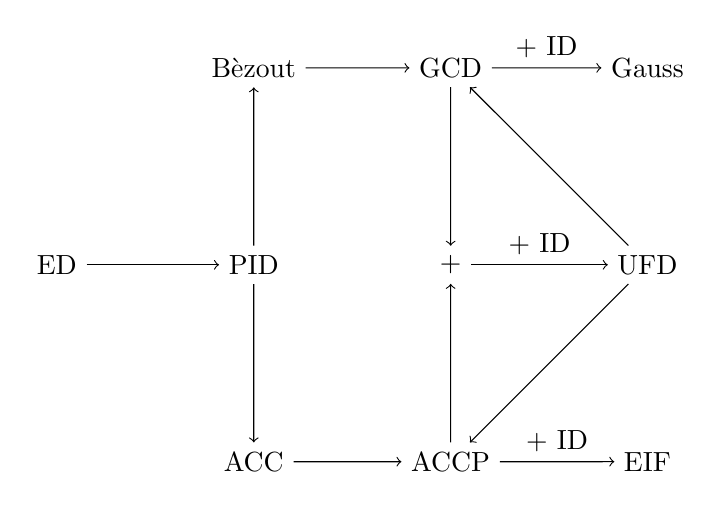
\begin{tikzpicture}[scale=2.5]
			\node (ED) at (0,0) {ED};
			\node (PID) at (1,0) {PID};
			\node (UFD) at (3,0) {UFD};
			\node (ACC) at (1,-1) {ACC};
			\node (ACCP) at (2,-1) {ACCP};
			\node (Bez) at (1,1) {Bèzout};
			\node (GCD) at (2,1) {GCD};
			\node (EIF) at (3,-1) {EIF};
			\node (Gau) at (3,1) {Gauss};
			\node (+1) at (2,0) {+};

			\draw[->] (ED) -- (PID);
			\draw[->] (ACCP) -- (+1);
			\draw[->] (GCD) -- (+1);
			\draw[->] (+1) -- node[above] {+ ID} (UFD);
			\draw[->] (UFD) -- (ACCP);
			\draw[->] (ACCP) -- node[above] {+ ID} (EIF);
			\draw[->] (PID) -- (Bez);
			\draw[->] (PID) -- (ACC);
			\draw[->] (ACC) -- (ACCP);
			\draw[->] (Bez) -- (GCD);
			\draw[->] (GCD) -- node[above] {+ ID} (Gau);
			\draw[->] (UFD) -- (GCD);
		\end{tikzpicture}
	\end{center}
	Da aggiungere: PID sse UFD + PRI => MXI, PID sse Bèzout + ACCP
	
	\section*{Definizioni}
	Nella nostra trattazione assumeremo che ED, PID, UFD non abbiano nella definizione il fatto di essere domini di integrità, scrivendo eventualmente dove serve.
	\begin{itemize}
		\item ({\bf ID - Integral Domain}) Un anello c.u. $R$ si dice dominio di integrità se vale $\forall a, b \in R \quad ab = 0 \implies a = 0 \opp b = 0$
		\item ({\bf ED - Euclidean Domain}) Un anello c.u. $R$ è detto dominio euclideo se $\exists \nu : R \setminus {0} \rar \bbN$ tale che $\forall a, b \in R \tc b \neq 0 \quad \exists q, r \in R \tc a = bq + r$ con $r = 0$ oppure $\nu(r) < \nu(b)$
		\item ({\bf PID - Principal Ideal Domain}) Un anello c.u. $R$ è detto ad ideali principali se ogni suo ideale è principale, ovvero è generato da un solo elemento. ($\forall I \subseteq R$ ideale si ha $\exists a \in R \tc I = (a)$)
		\item ({\bf UFD - Unique Factorization Domain}) Un anello c.u. $R$ è detto a fattorizzazione unica se $\forall r \in R \quad \exists ! p_1, \ldots, p_k \tc r = p_1 \ldots p_k$ con $p_i$ elemento irriducibile $\forall i$
		\item ({\bf ACC - Ascending Chain Condition}) Un anello c.u. $R$ è ACC se ogni catena ascendente infinita di ideali è stazionaria, ovvero se $I_1 \subseteq I_2 \subseteq \ldots \implies \exists n \tc I_k = I_n \forall k \ge n$
		\item ({\bf ACCP - Ascending Chain Condition on Principal ideals}) Un anello c.u. $R$ ha la proprietà delle catene ascendenti sugli ideali principali se non esiste una catena infinita strettamente ascendente di ideali principali, ovvero se $(a_1) \subseteq (a_2) \subseteq \ldots \implies \exists n \tc (a_k) = (a_n) \forall k \ge n$
		\item ({\bf EIF - Existence of Irreducible Factorization}) In anello c.u. $R$ esiste la fattorizzazione in irriducibili se ogni elemento si può scrivere (non necessariamente in modo unico) come prodotto di irriducibili, ovvero se $\forall r \in R \quad \exists a_1, \ldots, a_k \tc r = a_1 \ldots a_k$ con $a_i$ irriducibile $\forall i$
		\item ({\bf Bèzout}) Un anello c.u. $R$ è di Bèzout se ogni ideale finitamente generato è principale, ovvero se $I = (a_1, \ldots, a_k) \implies \exists \alpha \tc I = (\alpha)$
		\item ({\bf GCD - Greatest Common Divisor}) Se per ogni coppia di elementi esiste il massimo comun divisore, ovvero se $\forall a, b \in R \quad \exists d \in R \tc d \mid a, d \mid b$ e che $\forall h \in R \tc h \mid a, h \mid b \implies h \mid d$
		\item ({\bf Gauss}) Se vale il lemma di Gauss su $R[x]$
		\item ({\bf PRI - Prime Ideal}) Un ideale $I \subseteq R$ è detto primo se $I \neq (1)$ e se $xy \in I \implies x \in I \opp y \in I$
		\item ({\bf MXI - Maximal Ideal}) Un ideale $I \subseteq R$ è detto massimale se $I \neq (1)$ e se $\forall J \subseteq R$ ideale $\tc I \subseteq J$ si abbia $J = I \opp J = R$
		\item ({\bf PPI - Principal Ideal}) Un ideale $I \subseteq R$ si dice principale se è monogenerato, ovvero se $\exists a \in R \tc I = (a)$
	\end{itemize}

	\section*{Teoremi con dimostrazione}
	\subsection{Equivalenze di Ideali}
	\Enunciato
		$(i) \quad P $ PRI $\sse R/P$ è ID \\
		$(ii) \quad M $ MXI $\sse R/M$ è un campo \\
	\Dimostrazione Ovvie

	\subsection{ED $\implies$ PID}
	Sia $I \subseteq R$ ideale. Vogliamo mostrare che è principale. Si prenda un qualunque $a \in I \tc \nu(a)$ è la minima possibile tra gli elementi in $I$. Allora si ha (ED) $\forall b \in I \quad \exists q,r \in R \tc b = aq + r$, da cui segue $r = b - aq \in I$ e sappiamo che $r = 0 \opp \nu(r) < \nu(a)$, ma siccome $r \in I$, per come abbiamo scelto $a$, deve essere $r = 0$, ovvero $\forall b \in I \quad \exists q \in R \tc b = aq$, ovvero $I = (a)$
	
	\subsection{PID $\implies$ ACC}
	Sia $I_1 \subseteq I_2 \subseteq \ldots$ una catena ascendente di ideali. Vogliamo mostrare che è stazionaria. Definiamo $I := \cup_{i} I_i$ e notiamo che è un ideale. Allora si ha (PID) $I = (\alpha)$. Ma allora, poiché $\alpha \in I \implies \exists n \tc \alpha \in I_n$, ovvero essendo $I_n \subseteq I$ si ha $I_n = (\alpha)$, quindi $I_n = I_{n+1} = \ldots = I$

	\subsection{PID $\implies$ Bèzout}
	Essendo in un PID tutti gli ideali principali, lo sono anche quelli finitamente generati.

	\subsection{ACC $\implies$ ACCP}
	Ovvia, perché se vale su tutti gli ideali, vale in particolare anche sugli ideali principali.

	\subsection{ACCP + ID $\implies$ EIF}
	Dimostriamo che ogni elemento si scrive come prodotto di irriducibili. è chiaro che ogni elemento o è riducibile o non lo è. Sia quindi $a \in R$. Se $a$ è irriducibile abbiamo finito. Altrimenti $\exists a_1, b_1 \in R \tc a = a_1 b_1$. Ora, o entrambi sono irriducibili (e abbiamo finito) oppure almeno uno è riducibile. In particolare, o questo procedimento termina in un numero finito di passi (ovvero ci troviamo ad avere tutti elementi irriducibili ed abbiamo la tesi) oppure abbiamo sempre qualcuno riducibile. In particolare siano $a_1, a_2, \ldots$ quelli che possono sempre ridursi e $\tc a_i = b_{i+1}a_{i+1}$. Si consideri allora la catena ascendente $(a_1) \subseteq (a_2) \subseteq \ldots$ di ideali principali. Essa è stazionaria per ACCP, ovvero definitivamente $\exists k \tc (a_k) = (a_n) \forall n \ge k$, da cui segue $a_n = u_n a_k, a_k = v_n a_n$. E $a_k$ è irriducibile perché la decomposizione che avevamo trovato, ovvero $a_k = b_{k+1} a_{k+1} = b_{k+1} u_{k+1} a_k \implies 1 = b_{k+1} u_{k+1} \implies b_{k+1}$ invertibile, contraddicendo la riducibilità. Abbiamo quindi $a = a_1 \cdot \ldots \cdot a_k$ con tutti gli $a_i$ irriducibili.

	\subsection{Bèzout $\implies$ GCD}
	Dati $a, b \in R$ definiamo $d = \MCD(a,b) = \gen((a, b))$ come generatore dell'ideale generato da $a$ e $b$ (siccome sappiamo che ideali finitamente generati sono in realtà principali). Sicuramente $(a) \subseteq (a, b)$ e $(b) \subseteq (a, b)$, ovvero $d \mid a$ e $d \mid b$. Inoltre se $h \in R$ è $\tc h \mid a, h \mid b$ si ha $(a) \subseteq (h), (b) \subseteq (h) \implies (a, b) \subseteq (h)$, ovvero $(d) \subseteq (h)$, cioè $d \mid h$. Abbiamo quindi definito il $\MCD$ tra due elementi.

	\subsection{Lemmi sul GCD + ID}
	\Enunciato
		$(i)$ Supponiamo esistano $\MCD(a,b)$ e $\MCD(ac,bc)$. Allora vale $\MCD(ac,bc) = \MCD(a,b) c$ \\
		$(ii)$ Supponiamo $c \mid ab$ e $\MCD(a,c) = 1$. Allora $c \mid b$ \\
	\Dimostrazione
		$(i)$ Chiamiamo $d := \MCD(a,b)$. Chiaramente $cd \mid ca$, $cd \mid cb$, quindi $\MCD(ac, bc) = qcd$ per un qualche $q \in R$. Da cui segue $ac = qcdh$, $bc = qcdk$ per qualche $h, k$. Per cancellazione (ID) si ha $a = qdh$, $b = qdk$, quindi $qd \mid a, qd \mid b \implies qd \mid d \implies q$ invertibile, ovvero (siccome l'MCD è definito a meno di invertibili) si ha la tesi. \\
		$(ii)$ Notiamo che $c \mid cb$, ovvero $c \mid \MCD(ab,cb) = \MCD(a,c)b = b$, da cui la tesi.

	\subsection{GCD + ID $\implies$ Gauss}
	Definiamo contenuto di $f \in R[x]$ come $\MCD$ dei suoi coefficienti, ovvero se $f = \sum_{i=0}^{k} a_i x^i$, con $a_i \in R$, allora $c(f) := MCD(a_1, \ldots, a_k)$. Sia inoltre $F(R)$ il campo delle frazioni di $R$ e si indicherà con $\Lead(f)$ il termine di testa del polinomio $f$ \\
	\Enunciato
		$(i)$ Siano $f, g \in R[x]$. Allora vale $c(fg) = c(f) c(g)$, ovvero il contenuto è moltiplicativo. \\
		$(ii)$ Sia $f \in R[x]$ non costante, allora $f$ è irriducibile in $R[x]$ se e solo se è irriducibile in $F(R)[x]$ e primitivo in $R[x]$. \\
	\Dimostrazione
		$(i)$ Scritto $f = c(f) \sum_{i=0}^{n} \alpha_i x^i$ e $g = c(g) \sum_{j=0}^{m} \beta_j x^j$ si ha $fg = c(f) c(g) \sum_{k = 0}^{m+n} ( \sum_{i + j = k} \alpha_i \beta_j ) x^k$. Vorremmo mostrare $c(fg) = c(f)c(g)$, supponiamo WLOG $c(f) = c(g) = 1$. Se uno dei due polinomi $f, g$ ha al più un termine, il risultato è ovvio. Questo copre in particolare ogni caso con meno di quattro termini nonzero. Assumiamo ora quindi che sia $f$ che $g$ abbiano grado almeno due e che il risultato sia dimostrato per tutti i polinomi con un numero minore di termini. Allora se il contenuto $C := c(fg)$ non è invertibile, ha un divisore non banale in comune con il coefficiente del termine di testa di almeno uno tra $f$ e $g$ (siccome divide il loro prodotto, che è il coefficiente di testa di $fg$). WLOG supponiamo $d = \MCD(C,\Lead(f)) \neq 1$. Siccome $d \mid fg$, $d \mid \Lead(f)g$ si ha $d \mid (f - \Lead(f))g$, cioè divide il suo contenuto, che per induzione ($(f - \Lead(f))g$ è di grado minore di $fg$) è $c(f - \Lead(f))c(g) = c(f - \Lead(f))$. Siccome $d$ divide anche $c(\Lead(f))$, divide anche $c(f) = 1$, quindi $d$ era invertibile $\implies C$ invertibile. Ovvero vale $c(fg) = c(f)c(g)$ \\
		$(ii)$ \frsx Ovvia (infatti se abbiamo una fattorizzazione in $R[x]$ ed il polinomio è primitivo, allora la fattorizzazione si trasporta anche in $F(R)[x]$ con gli stessi polinomi, che hanno grado positivo). \\
		$(ii)$ \frdx Proviamo che se $f$ ha grado positivo ed è irriducibile in $R[x]$ allora è irriducibile anche in $F(R)[x]$. Notiamo che in $F(R)[x] \setminus \{0\}$ ogni classe di elementi associati (ovvero relazionati da moltiplicazione per un elemento non-zero del campo $F(R)$) incontra l'insieme degli elementi primitivi in $R[x]$: a partire da un arbitrario elemento della classe, uno può prima moltiplicare per un elemento diverso da zero di $R$ per togliere i denominatori ed entrare in $R[x]$, poi può dividere per il MCD dei coefficienti per ottenere un polinomio primitivo. Ora assumiamo che $f$ sia riducibile in $F(R)[x]$, ovvero $f = gh$, con $g, h \in F(R)[x]$ non costanti. Possiamo rimpiazzare $g, h$ da elementi associati e ottenere $f = \alpha g' h'$, per qualche $\alpha \neq 0 \in F(R)$. Ma $g'h'$ è primitivo in $R[x]$ per il punto $(i)$, quindi $\alpha \in R$ (Se $\alpha$ si scrive come frazione $\frac{a}{b}$, allora $b$ deve dividere tutti i coefficienti di $ag'h'$, quindi $b \mid c(ag'h') = a$, che significa $\alpha \in R$) e la decomposizione $f = \alpha g'h'$ contraddice l'irriducibilità di $f$ in $R[x]$.

	\subsection{Relazioni tra Primo ed Irriducibile}
	\Enunciato
		$(i)$ (ID) Primo $\implies$ Irriducibile \\
		$(ii)$ (GCD + ID) Irriducibile $\implies$ Primo \\
	\Dimostrazione
		$(i)$ Sia $p \in R$ primo. E supponiamo che $p = ab$, allora $p \mid ab \implies p \mid a \opp p \mid b$. WLOG supponiamo $p \mid a$, allora $a = kp$, ovvero $p = ab = kpb \implies 1 = kb$, quindi $b$ è invertibile, contro le ipotesi. \\
		$(ii)$ Sia $r \in R$ irriducibile. Supponiamo $r \mid ab$. Allora si ha $\MCD(r,a) = 1 \opp r$ perché $r = \MCD(r,a) k$ e $k$ invertibile, oppure $\MCD(r,a)$ invertibile. Se $\MCD(r,a) = 1$ si ha (Lemma ii su GCD+ID) $r \mid b$, se invece $\MCD(r,a) = r$ si ha $r \mid a$, da cui la tesi. \\

	\subsection{GCD + ID + ACCP $\implies$ UFD}

	\subsection{UFD $\implies$ ACCP}

	\subsection{UFD $\implies$ GCD}

	\section*{Cosa passa a strutture create da $R$}
	
	\begin{tabular}{lccccc}
	 & {\bf Sottoanelli} & {\bf Ideali} & {\bf Quozienti} & {\bf $R[x]$} & {\bf Localizzazione} \\
	{\bf ID} & \checkmark & \checkmark & & \checkmark & \\
	{\bf ACC} & & & & \checkmark & \\
	{\bf ACCP} & & & & \checkmark & \\
	{\bf GCD + ID} & & & & \checkmark & \\
	{\bf UFD + ID} & & & & \checkmark & \\
	{\bf PID} & & & & \crossmark & \\
	{\bf ED} & & & & \crossmark & \\
	{\bf Bèzout} & & & & & \\
	
	\end{tabular} \vskip 1cm

	
	\subsection{Cosa passa ad R[x]}
	\Enunciato
		$(i)$ $R$ ID $\implies R[x]$ ID \\
		$(ii)$ $R$ GCD + ID $\implies R[x]$ GCD + ID \\
		$(iii)$ $R$ ACC $\implies R[x]$ ACC \\
		$(iv)$ $R$ ACCP $\implies R[x]$ ACCP \\
		$(v)$ $R$ UFD + ID $\implies R[x]$ UFD + ID \\

	\Dimostrazione
		$(i)$ Supponiamo per assurdo che $fg = 0 \in R[x]$, con $f, g \neq 0$, allora si ha, prendendo il termine di testa, che $\Lead(f)\Lead(g) = \Lead(0)$, ovvero $\alpha x^n \beta x^m = 0 \implies \alpha \beta = 0$ con $\alpha, \beta \neq 0$ quindi si ha che $R$ non è ID, assurdo. \\
		$(ii)$ \\
		$(iii)$ \\
		$(iv)$ Segue dalle precedenti: $R$ UFD + ID $\sse R$ GCD + ID + ACCP $\implies R[x]$ GCD + ID + ACCP $\sse R[x]$ UFD + ID \\


	\subsection{Cosa passa ai sottoanelli}
	\Enunciato
		$(i)$ $R$ ID e $S \subseteq R \implies S$ ID \\

	\Dimostrazione
		$(i)$ Ovvio perché le definizioni sono quantificate con $\forall$ e continuano a valere anche se ci restringiamo ad un insieme più piccolo.

	\subsection{Cosa passa gli ideali}

	\subsection{Cosa passa agli anelli quoziente}

	\subsection{Cosa passa all'anello localizzato}

\end{document}
